\documentclass[mathserif,hyperref={pdfpagemode=FullScreen}]{beamer}
% \documentclass[handout]{beamer}
% \usetheme{Dresden}
\usetheme{340}
\beamertemplatetransparentcovereddynamic
\usepackage[latin1]{inputenc}
\usepackage{pgf}
\usepackage{multirow}
\usepackage{comment}
\usepackage{epsfig,color}
\usepackage{hyperref}
% \usepackage{algorithm}
\usepackage{algorithmic}
\usepackage{amsmath,color}

\usepackage{tcolorbox}
%\usepackage{wasysym}
\usepackage{tikz}
\usepackage[export]{adjustbox}

%\usepackage{subfig}
%\usepackage{colortbl}
%\usepackage{array}
\usepackage{booktabs}
%\usepackage{floatrow}
%\usepackage{balance}

\usepackage{float}
\usepackage{tikz}

%%\usepackage{enumitem}
%%\setlist[description]{leftmargin=*}

\usetikzlibrary{patterns}
\usetikzlibrary{fit,calc,positioning,decorations.pathreplacing,matrix}
\tikzset{xtick/.style={inner xsep=0pt, inner ysep=3pt, minimum
		size=0pt, draw, label=below:#1},%
	comm/.style args={#1start#2length#3color#4}{rounded corners=1mm, draw, inner
		sep=0pt, fill=#4, label=center:#1, fit={(#2,0.75)
			(#2+#3,1.5)}},%
	comp/.style args={#1start#2length#3color#4}{rounded corners=1mm, draw, inner
		sep=0pt, fill=#4, label=center:#1, fit={(#2,0)
			(#2+#3,0.75)}},%
}

\newcommand{\schedule}[3]{
	\draw[->] (-0.2, 0) -- (#1, 0) node[below] {$t$};
	\draw (0, 0) -- (0, 1.5);
	\node at (-0.8, 0.75)[rotate=90] {#2};
	\draw[dashed,gray] (0, 0.75) -- (#1, 0.75);
	\foreach \t in {0,#3} {
		\node[xtick=\t] at (\t, 0){};
	}
}
\newcommand{\task}[6][0]{
	\node[comm=#2 start #3 length #4 color #6]{};
	\node[comp=#2 start #3+#4+#1 length #5 color #6]{}; 
}


\newcommand{\continue}{{\bf continue}}

\newcommand{\gem}{{\sc dgemm}\xspace}
\newcommand{\trsm}{{\sc dtrsm}\xspace}
\newcommand{\potrf}{{\sc dpotrf}\xspace}
\newcommand{\syrk}{{\sc dsyrk}\xspace}




\newcommand{\tto}{ {T}_{\textsc FirstIdle}\xspace}
%\newcommand{\ttG}{ {T}_{\textsc GPUNoSpoliation}\xspace}
%\newcommand{\ttC}{ {T}_{\textsc CPUNoSpoliation}\xspace}
%%\newcommand{\HEG}{{\textsc HP}_{\textsc GPU}\xspace}
%\newcommand{\HEC}{{\textsc HP}_{\textsc CPU}\xspace}
%\newcommand{\HE}{{\textsc HP}_{\textsc MakeSpan}\xspace}
\newcommand{\HE}{C_{\max}^{\textsc HP}\xspace}

%\newcommand{\WC}{ {\sc W}_{\textsc CPU}\xspace}
%\newcommand{\WG}{ {\sc W}_{\textsc GPU}\xspace}
%\newcommand{\AG}{ {\cal A}_{\textsc GPU}\xspace}
%\newcommand{\AC}{ {\cal A}_{\textsc CPU}\xspace}
\newcommand{\copt}{{C_{\max}^{\textsc Opt}}\xspace}
\newcommand{\abd}{{AreaBound}\xspace}
%\newcommand{\wls}{{WorstListSchedule}\xspace}

\newcommand{\I}{{\cal I}\xspace}

\newcommand{\hpsched}{\ensuremath{{\cal S}_{\text{HP}}}\xspace}
\newcommand{\hpschedns}{\ensuremath{{\cal S}_{\text{HP}}^{\text{NS}}}\xspace}


\newcommand{\mkl}{{\sc Mkl}\xspace}
\newcommand{\pmkl}{{\sc Parallel Mkl}\xspace}
\newcommand{\maphys}{{\sc MaPHyS}\xspace}
\newcommand{\pdslin}{{\sc PDSLin}\xspace}
%%\newcommand{\superlu}{{\sc SuperLU\_D\IST}\xspace}
\newcommand{\hips}{{\sc Hips}\xspace}
%%\newcommand{\shylu}{{\sc ShyLU}\xspace}
%%\newcommand{\pastix}{{\sc PaStiX}\xspace}
%%\newcommand{\mumps}{{\sc Mumps}\xspace}
%%\newcommand{\pardiso}{{\sc Pardiso}\xspace}
%%\newcommand{\scotch}{{\sc Scotch}\xspace}
%%\newcommand{\metis}{MET\IS\xspace}
%%\newcommand{\chameleon}{{\sc Chameleon}\xspace}
%%\newcommand{\hwloc}{hwloc\xspace}
%%\newcommand{\plasma}{{\sc Plasma}\xspace}
%%\newcommand{\magma}{{\sc Magma}\xspace}
%%\newcommand{\cublas}{{\sc cuBLAS}\xspace}
%%\newcommand{\dplasma}{DPLASMA\xspace}
%%\newcommand{\qrm}{\texttt{qr\_mumps}\xspace}
%%\newcommand{\qrs}{\texttt{qrm\_starpu}\xspace}
%%\newcommand{\qrp}{\texttt{qrm\_parsec}\xspace}
%%\newcommand{\spqr}{\texttt{spqr}\xspace}
%%\newcommand{\lws}{{\sc lws}\xspace}
%%\newcommand{\quark}{{QUARK}\xspace}
%%\newcommand{\starpu}{{StarPU}\xspace}
%%\newcommand{\starss}{{StarSs}\xspace}
%%\newcommand{\parsec}{{PaRSEC}\xspace}
%%\newcommand{\simgrid}{{SimGrid}\xspace}
%%\newcommand{\openmp}{{OpenMP}\xspace}
%%\newcommand{\stf}{{STF}\xspace}
%%\newcommand{\ptg}{{PTG}\xspace}
\newcommand{\heftp}{\emph{heftp}\xspace}
%%\newcommand{\heteroprio}{{HeteroPrio}\xspace}
\newcommand{\heteroprio}{{HeteroPrio}\xspace}
\newcommand{\spoliation}{{spoliation}\xspace}
\newcommand{\preemption}{{preemption}\xspace}





\date{\includegraphics[width=.25\linewidth]{icpp.png}\\August 8, 2019}
\newcommand{\highlight}[1]{\colorbox{red}{$\displaystyle #1$}}
\pdfcompresslevel=2             %-- 0 = none, 9 = best

\input{common.tex}

\title[Performance Models for Data Transfers: A Case Study]{Performance Models for Data Transfers: A Case Study with Molecular Chemistry Kernels}
%% \author[{\sc Inria Bordeaux}]{Olivier {\sc Beaumont}, 
%% Lionel {\sc Eyraud-Dubois}, and\\ \underline{Suraj {\sc Kumar}}
%%%\author[{\sc Inria}]{Suraj {\sc Kumar}
%%%%\author[shortname]{author1 \inst{1} \and author2 \inst{2}}
%%%%\institute[shortinst]{\inst{1} affiliation for author1 \and %
%%%%	\inst{2} affiliation for author2}
%%} 
\author[ICPP-2019]{\underline{Suraj {\sc Kumar}}\inst{1}, Lionel {\sc Eyraud-Dubois}\inst{2}, and\\ Sriram {\sc Krishnamoorthy}\inst{1}}
\institute[shortinst]{\inst{1} Pacific Northwest National Laboratory, Richland, USA\and %
	\inst{2} Inria Bordeaux -- Sud-Ouest, France} 



%%Suraj Kumar (Paci c Northwest National Laboratory), Lionel Eyraud-Dubois (Inria Bordeaux Sud- Ouest), Sriram Krishnamoorthy (Paci c Northwest National Laboratory)

\vfill
%\logo{
%
\includegraphics[width=.3\linewidth]{logo/logo_inria}
%~~~~~~~~~~~~~~~~~~~~~~~~~~~~~~~~~~~~~
%~~~~~~~~~~~~~~~~~~~~~~~~~~~~~~~~~~~~~
%%\raisebox{0.5cm}{
\includegraphics[width=.20\linewidth]{logo/logo_labri}}
%% 
\includegraphics[width=.3\linewidth]{logo_labri}
%\hfill
%~~~~~~~~~~~~~~~~~~~~~~~~~~~~~~~~~~~~~
%~~~~~~~~~~~~~~~~~~~~~~~~~~~~~~~~~~~~~
%\includegraphics[width=.3\linewidth]{logo/logo_UBordeaux}
%}

\logo{%
	\makebox[0.95\paperwidth]{%
		\includegraphics[width=.3\linewidth]{logo_pnnl.png}
		\hfill%
		
\includegraphics[width=.3\linewidth]{logo_inria.png}
	}%
}

% \date{\small Inria Team\\~\\~\\~\\}
% first argument: slide number to appear from, second argument: content of header 
\newcommand{\hiddencell}[2]{\action<#1->{#2}}
\begin{document}

% Page de garde
\frame{\titlepage}
\logo{}





%%\frame{
%%  \frametitle{Outline}
%%  \tableofcontents
%%}
%%\begin{frame}[fragile]{Test}
%%%%	\begin{figure}
%%	\begin{tikzpicture}
%%	\schedule{24}{}{4,8,10,20}
%%	\end{tikzpicture}
%%	\begin{block}{title}
%%	\newcommand{\taskA}[1]{\node[comp=$A$ start #1 length 5 color cyan] {};}
%%\newcommand{\taskB}[2][0]{\task[#1]{$B$}{#2}{4}{3}{blue!25!white}}
%%\newcommand{\taskC}[2][0]{\task[#1]{$C$}{#2}{1}{6}{blue!50!white}}
%%\newcommand{\taskD}[2][0]{\task[#1]{$D$}{#2}{3}{7}{blue!75!white}}
%%\newcommand{\taskE}[2][0]{\node[comm=$E$ start #2 length 6 color green!25!white]{};%
%%	\node[comp={} start #2+6+#1 length 0.5 color green!25!white]{};}
%%\newcommand{\taskF}[2][0]{\node[comm=$F$ start #2 length 7 color green!50!white]{};%
%%	\node[comp={} start #2+7+#1 length 0.5 color green!50!white]{};}
%%\begin{tikzpicture}[yscale=0.7, thick, xscale=0.3]
%%\schedule{24}{}{5,8,15,21.5,23}
%%\taskA{0}
%%\taskB[1]{0}
%%\taskD[1]{4}
%%\taskE[1]{8}
%%\taskC[0.5]{14}
%%\taskF{15.5}
%%\end{tikzpicture}
%%	\end{block}
%%%%\end{figure}
%%\end{frame}


%%%%%%%%%%%%%%
\section{Introduction} 
\begin{frame}{Introduction}
 \begin{itemize}
 	\vfill
  \item Distributed memory systems are very common
  \vfill
 \item Rate of computation vs rate of data movement
 \vfill
  \item Focus: Avoid, Hide, and Minimize communication costs
  \vfill

 \end{itemize}
\end{frame}

\begin{frame}{Task Graphs and Runtime Systems}
%%   \begin{itemize}
%%   	 \item Applications can be expressed as task graphs
%%\end{itemize}
		\begin{columns}
	\null \hfill
	\begin{column}{0.4\linewidth}
		\begin{center}
			\includegraphics[scale=0.2]{diagrams/taskGraph.eps}
		\end{center}
	\end{column}
	\begin{column}{0.5\linewidth}
		\begin{itemize}
			   	 \item Applications can be expressed as task graphs
			   	 \item Vertices represent tasks
			   	 \item Edges represent dependencies among tasks
		\end{itemize}
	\end{column}
\end{columns}
%%		\begin{center}
%%	\includegraphics[scale=0.2]{diagrams/taskGraph.eps}
%%\end{center}
\begin{block}{Task Based Runtime Systems}
		\begin{itemize}
	\item StarPU, QUARK, PaRSEC, StarSs, Legion, KAAPI
%%	\item Manages scheduling of computations and communications
	\item May only see a set of ready (independent) tasks
	\item A memory node may require data from other memory nodes 
%%	\item Output data is managed by runtime based on demand 

	\only<1>{ \item Order of data transfers such that communication-computation overlap is maximized}
	\only<2>{\item Order of data transfers \textcolor{red}{between two memory nodes} such that communication-computation overlap is maximized}
\end{itemize}
\end{block}

\end{frame}

\section{Problem Definition}
\begin{frame}{Problem Definition}
\begin{itemize}
	\item Communication and computation times are known in advance
	\begin{itemize}
		\item Approximated based on number of computations and hardware details
		\item Obtained from previous executions
	\end{itemize}
%%\item Tasks do not produce output data (or store in a separate buffer)
\end{itemize}
\begin{block}{Problem $DT$ }
	\begin{itemize}
		\item A set of tasks $ST=\{T_1, \cdots, T_n\}$ is scheduled on a processing unit $P$ with
		memory unit $M$ of capacity $C$
		\item Input data for tasks of $ST$
		reside on another memory unit
		\item Tasks do not produce output data
		\item Tasks do not require intermediate memory
		\item A tasks uses an amount of memory in $M$ from the
		start of its communication to the end of its computation
	\end{itemize}
\noindent Given $L$, is there a feasible schedule $S$ for $ST$ such that
makespan of $S$, $\mu(S) \le L$?
\end{block}

\end{frame}

\begin{frame}{Relevant Problem in Literature}
\begin{block}{Machine Flowshop Problem}
	\begin{itemize}
		\item $n$ machines and $m$ tasks 
		\item Each task contains exactly $n$ operations
		\item $i$-th operation of a task must be processed on the $i$-th machine
		\item Each machine can perform at-max one operation at a time
		\item $i$-th operation of a task starts after the completion of $(i-1)$-th operation
	\end{itemize}
	The problem is to obtain the arrangement that achieves shortest possible makespan.
\end{block}

\begin{block}{}
	\begin{itemize}
		\item 	Johnson provided an optimal algorithm for 2-machine flow shop problem
		\item Our  problem $DT$ adds one extra dimension (memory capacity) to 2-machine flowshop problem
	\end{itemize}
\end{block}

\end{frame}

\subsection{Unlimited Memory Capacity}

\begin{frame}
	\frametitle{Table of Contents}
	\tableofcontents[currentsubsection]
\end{frame}

\newcommand{\scomm}{\ensuremath{{S}_{\text{COMM}}}}
\newcommand{\scomp}{\ensuremath{{S}_{\text{COMP}}}}

\begin{frame}{Unlimited Memory Capacity}{Johnson's Algorithm}
\begin{algorithm}[H]
\begin{algorithmic}[1]
	\STATE Divide ready tasks in two sets $S_1$ and $S_2$. If computation time of a task $T$ is not less than its communication time, then $T$ is in $S_1$ otherwise in $S_2$.
	\STATE Sort $S_1$ in queue $Q$ by non-decreasing communication times
	\STATE Sort $S_2$ in queue $Q'$ by non-increasing computation times
	\STATE Append $Q'$ to $Q$
	\STATE $\tau_{\text{COMM}} \gets 0$ \hfill\COMMENT{Available time of communication resource}
	\STATE $\tau_{\text{COMP}} \gets 0$\hfill \COMMENT{Available time of computation resource}
	\WHILE{$Q \neq \emptyset$}
	\STATE Remove a task $T$ from beginning of $Q$ for processing
	\STATE $\scomm(T) \gets \tau_{\text{COMM}}$
	\STATE $\scomp(T) \gets max(\scomm(T) + COMM_T, \tau_{\text{COMP}})$
	\STATE $\tau_{\text{COMM}} \gets \scomm(T) + COMM_T$
	\STATE $\tau_{\text{COMP}} \gets \scomp(T) + COMP_T$
	\ENDWHILE
\end{algorithmic}
\end{algorithm}
$\bullet$ $OMIM$ denotes the makespan of this algorithm
\end{frame}


\begin{frame}{Approach for the optimality proof}
\vspace*{-0.5cm}
\begin{center}
\includegraphics[scale=0.32]{./diagrams/original_swapped_schedules-eps-converted-to.pdf}
\end{center}

\end{frame}






\subsection{Limited Memory Capacity}
\begin{frame}
\frametitle{Table of Contents}
\tableofcontents[currentsubsection]
\end{frame}
\newcommand{\threepart}{\textsc{3Par}\xspace}
\begin{frame}{Limited Memory Capacity}
\begin{itemize}
	\item Memory is required only to store input data (from the definition of our problem)
	\item As Communication time $\propto$ amount of communication, for each task:
	\begin{itemize}
		\item Communication time = Amount of communication  (\textcolor{green}{for simplification})
		\item Communication time = Amount of input data
	\end{itemize}
\end{itemize}

\begin{block}{Reduction Problem}
\textbf{Three Partition Problem} (\threepart): Given a set of
$3m$ integers $A = \{ a_1, \cdots, a_{3m }\}$, is there a partition
of $A$ into $m$ triplets $TR_i = \{a_{i_1}, a_{i_2}, a_{i_3}\}$,
such that $\forall i, a_{i_1} + a_{i_2} + a_{i_3} = b$, where
$b=(1/m) \sum a_i $?
\end{block}
\end{frame}

\begin{frame}{Reduction: \threepart to $DT$ }
\begin{block}{Definition of tasks in the reduction from \threepart}

 $\qquad x = max\{a_i:1\le i\le 3m\}$
\begin{center}
\begin{tabular}{ |c|c|c| }
	\hline
	Task & Communication time & Computation time \\ \hline
	$K_0$ & $0$ & $3$ \\ \hline
	$K_1, \cdots, K_{m-1}$ & $b'=b+6x$ & $3$\\ \hline
	$K_m$ & $b'=b+6x$ & $0$ \\ \hline
	$1\le i \le 3m, A_i$ & $1$ & $a_i' = a_i + 2x$\\ \hline
\end{tabular}
\end{center}
\begin{center}
\noindent Total memory capacity: $C=b'+3$\\
\noindent Target makespan: $L=m(b'+3)$
\end{center}
\end{block}
\end{frame}



\begin{frame}[fragile]{Pattern of Feasible Schedule}
\tikzset{xtick/.style={inner xsep=0pt, inner ysep=3pt, minimum size=0pt, draw},%
	task/.style args={#1start#2length#3res#4color#5}{rounded corners, draw, inner
		sep=0pt, fill=#5, label=center:#1, fit={(#2,#4*0.75) (#2+#3,#4*0.75+0.75)}},%
	vert/.style={inner sep=1pt, fill=black, circle, draw, label=#1}
}
\newcommand{\scheduleNoName}[1]{
	\draw[->] (-0.4, 0) -- (#1, 0) node[below] {$t$};
	\draw (0, 0) -- (0, 1.5) node[pos=0.25, left] {Comp.}
	node[pos=0.75, left] {Comm.};
	\draw[dashed,gray] (0, 0.75) -- (#1, 0.75);
}
%%		\begin{figure}[htb]
%%	\centering
\begin{center}
	\begin{tikzpicture}[yscale=0.7, thick, xscale=0.6]
	\scheduleNoName{12.5}
	\node[task=$A_{1,1}$ start 0 length 1 res 1 color cyan]{};
	\node[task=$A_{1,2}$ start 1 length 1 res 1 color blue!40!white]{};
	\node[task=$A_{1,3}$ start 2 length 1 res 1 color blue!70!white]{};
	\node[task=$K_0$ start 0 length 3 res 0 color gray!40!white]{};
	\node[task=$K_1$ start 3 length 6 res 1 color green]{}; 
	\node[task=$A_{1,1}$ start 3 length 1.8 res 0 color cyan]{};
	\node[task=$A_{1,2}$ start 4.8 length 2.3 res 0 color blue!40!white]{};
	\node[task=$A_{1,3}$ start 7.1 length 1.9 res 0 color blue!70!white]{};
	\node[task=$A_{2,1}$ start 9 length 1 res 1 color cyan]{};
	\node[task=$A_{2,2}$ start 10 length 1 res 1 color blue!40!white]{};
	\node[task=$A_{2,3}$ start 11 length 1 res 1 color blue!70!white]{};
	\node[task=$K_1$ start 9 length 3 res 0 color green]{};
	\draw[<->,thin] (0, -0.2) -- node[below]{$3$} (3, -0.2) ;
	\draw[<->,thin] (9, -0.2) -- node[below]{$3$} (12, -0.2) ;
	\draw[<->,thin] (3, -0.2) -- node[below]{$b'$} (9, -0.2) ;
	\end{tikzpicture}
\end{center}
	\begin{block}{}
		\begin{itemize}
			\item Problem $DT$ is NP-Complete.
			\item Our proof is inspired from  work  by Papadimitriou et al. (on 2-machine flowshop  with limited buffer problem)
		\end{itemize}
	\end{block}
%%\end{figure}
\end{frame}

\setlength{\tabcolsep}{3pt}

\begin{frame}[fragile]{Order of Processing on Communication and Computation Resources in Optimal Schedules}
\begin{columns}

	
	\begin{column}[c]{.35\linewidth}
		\footnotesize
		\begin{center}
\begin{tabular}{|c|c|c|c|}
	\hline
	Task & Memory & Comm & Comp\\
	& Req & Time & Time\\ \hline 
	%%				\multirow{2}{*}{Task} & Memory Req & \multirow{2}{*}{Comm Time} & \multirow{2}{*}{Comp Time}\\  
	%%				&=Comm Volume && \\ \hline
	A & 0 & 0 & 5\\ \hline
	B & 4 & 4 & 3\\ \hline
	C & 1 & 1 & 6\\ \hline
	D & 3 & 3 & 7\\ \hline
	E & 6 & 6 & 0.5\\ \hline
	F & 7 & 7 & 0.5\\ \hline
\end{tabular}
		\end{center}
	\end{column}

	\newcommand{\taskA}[1]{\node[comp=$A$ start #1 length 5 color cyan] {};}
	\newcommand{\taskB}[2][0]{\task[#1]{$B$}{#2}{4}{3}{blue!25!white}}
	\newcommand{\taskC}[2][0]{\task[#1]{$C$}{#2}{1}{6}{blue!50!white}}
	\newcommand{\taskD}[2][0]{\task[#1]{$D$}{#2}{3}{7}{blue!75!white}}
	\newcommand{\taskE}[2][0]{\node[comm=$E$ start #2 length 6 color green!25!white]{};%
	\node[comp={} start #2+6+#1 length 0.5 color green!25!white]{};}
	\newcommand{\taskF}[2][0]{\node[comm=$F$ start #2 length 7 color green!50!white]{};%
	\node[comp={} start #2+7+#1 length 0.5 color green!50!white]{};}




	\begin{column}[c]{.65\linewidth}
%%%%	\begin{figure}[!htb]
%%	\centering
\footnotesize
	\begin{block}{Common ordering on both
			resources}
%%\renewcommand{\schedule}[3]{
%%	\draw[->] (-0.2, 0) -- (#1, 0) node[below] {$t$};
%%	\draw (0, 0) -- (0, 1.5);
%%	\node at (-0.8, 0.75)[rotate=90] {#2};
%%	\draw[dashed,gray] (0, 0.75) -- (#1, 0.75);
%%	\foreach \t in {0,#3} {
%%		\node[xtick=\t] at (\t, 0){};
%%	}
%%}
\begin{tikzpicture}[yscale=0.7, thick, xscale=0.3]
\schedule{24}{}{5,8,15,21.5,23}
\taskA{0}
\taskB[1]{0}
\taskD[1]{4}
\taskE[1]{8}
\taskC[0.5]{14}
\taskF{15.5}
\end{tikzpicture}
	\end{block}
\begin{block}{Different ordering on both
		resources}
\begin{tikzpicture}[yscale=0.7, thick, xscale=0.3]
\schedule{24}{}{5,8,14,22}
\taskA{0}
\taskB[1]{0}
\taskC[3]{4}
\taskD[6.5]{5}
\taskE{8}
\taskF{14.5}
\end{tikzpicture}
\end{block}
%%%%	\caption{Schedules for the instance ofTable~\ref{table:different.order} with a memory capacity of 10.\vspace*{-0.75cm}}
%%\end{figure}
	\end{column}
\end{columns}
\end{frame}

\section{Classes of Heuristics}
\begin{frame}
\frametitle{Table of Contents}
\tableofcontents[currentsection]
\end{frame}

\begin{frame}{Our Heuristics}
\begin{itemize}
	\vfill
	\item Static order based strategies
	\vfill
	\item Dynamic selection based strategies
	\vfill
	\item Static order with dynamic correction based strategies
	\vfill
\end{itemize}
We consider common order on both resources for all of our heuristics.
\end{frame}
\subsection{Static Order Based Strategies}
\begin{frame}{Static Order Based Strategies}
\begin{itemize}
	\vfill
	\item \textit{order of optimal strategy infinite memory} ($OOSIM$)
	\vfill
	\item \textit{increasing order of communication strategy} ($IOCMS$)
	\vfill
	\item \textit{decreasing order of computation strategy} ($DOCPS$)
	\vfill
	\item \textit{increasing order of communication plus computation strategy} ($IOCCS$)
	\vfill
	\item \textit{decreasing order of communication plus computation strategy} ($DOCCS$)
	\vfill
\end{itemize}
\end{frame}
\begin{frame}[fragile]{Static Order Based Strategies}
\begin{columns}
	\footnotesize
\begin{column}[c]{0.4\linewidth}
	\begin{tabular}{|c|c|c|c|}
		\hline
	Task & Memory & Comm & Comp\\
& Req & Time & Time\\ \hline 
		A & 3 & 3 &  2\\ \hline
		B & 1 & 1 & 3\\ \hline
		C & 4 & 4 & 4\\ \hline
		D & 2 & 2 & 1\\ \hline
	\end{tabular}
\vspace*{0.5cm}
\begin{block}{Unlimited Memory Capacity}
	\newcommand{\taskA}[2][0]{\task[#1]{$A$}{#2}{3}{2}{cyan}}
	\newcommand{\taskB}[2][0]{\task[#1]{$B$}{#2}{1}{3}{blue!40!white}}
	\newcommand{\taskC}[2][0]{\task[#1]{$C$}{#2}{4}{4}{blue!70!white}}
	\newcommand{\taskD}[2][0]{\task[#1]{$D$}{#2}{2}{1}{blue}}
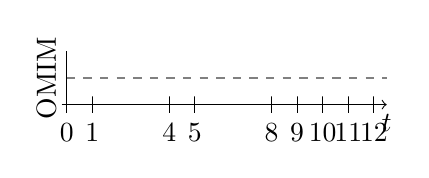
\begin{tikzpicture}[yscale=0.45, xscale=0.325]
\schedule{12.5}{OMIM}{1,4,5,8,9,10,11,12}
\taskB{0}
\taskC{1}
\taskA[1]{5}
\taskD[1]{8}
\end{tikzpicture}
\end{block}
\end{column}
\begin{column}[c]{0.6\linewidth}
	\begin{block}{Memory Capacity: 6}
	\newcommand{\taskA}[2][0]{\task[#1]{$A$}{#2}{3}{2}{cyan}}
	\newcommand{\taskB}[2][0]{\task[#1]{$B$}{#2}{1}{3}{blue!40!white}}
	\newcommand{\taskC}[2][0]{\task[#1]{$C$}{#2}{4}{4}{blue!70!white}}
	\newcommand{\taskD}[2][0]{\task[#1]{$D$}{#2}{2}{1}{blue}}
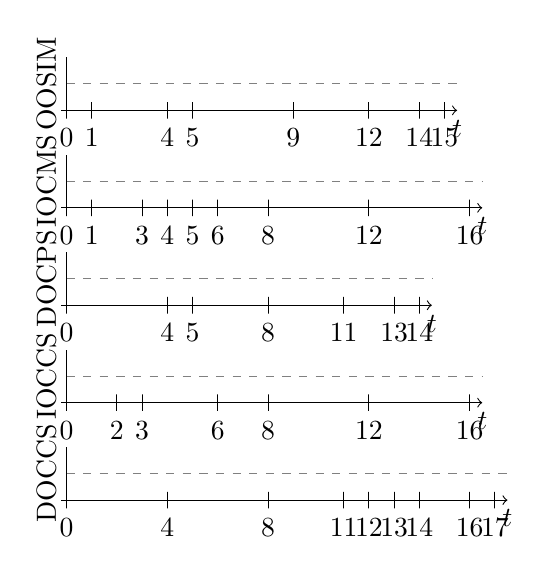
\begin{tikzpicture}[yscale=0.45, xscale=0.32]
\begin{scope}
\schedule{15.5}{OOSIM}{1,4,5,9,12,14,15}
\taskB{0}
\taskC{1}
\taskA{9}
\taskD{12}
\end{scope}
\begin{scope}[yshift=-2.75cm]
\schedule{16.5}{IOCMS}{1,3,4,5,6,8,12,16}
\taskB{0}
\taskD[1]{1}
\taskA{3}
\taskC{8}
\end{scope}
\begin{scope}[yshift=-5.5cm]
\schedule{14.5}{DOCPS}{4,5,8,11,13,14}
\taskC{0}
\taskB[3]{4}
\taskA{8}
\taskD{11}
\end{scope}
\begin{scope}[yshift=-8.25cm]
\schedule{16.5}{IOCCS}{2,3,6,8,12,16}
\taskD{0}
\taskB{2}
\taskA{3}
\taskC{8}
\end{scope}
\begin{scope}[yshift=-11cm]
\schedule{17.5}{DOCCS}{4,8,11,12,13,14,16,17}
\taskC{0}
\taskA{8}
\taskB[1]{11}
\taskD[2]{12}
\end{scope}
\end{tikzpicture}
	\end{block}
\end{column}
\end{columns}
\end{frame}

\subsection{Dynamic Selection Based Strategies}
\begin{frame}{Dynamic Selection Based Strategies}
\begin{itemize}
	\vfill
	\item \textit{largest communication task respects memory restriction} ($LCMR$)
	\vfill
	\item \textit{smallest communication task respects memory restriction} ($SCMR$)
	\vfill
	\item \textit{maximum accelerated task respects memory restriction} ($MAMR$)
	\vfill
\end{itemize}
\end{frame}

\begin{frame}[fragile]{Dynamic Selection Based Strategies}
\begin{columns}
	\footnotesize
	\begin{column}[c]{0.4\linewidth}
		\begin{tabular}{|c|c|c|c|}
			\hline
	Task & Memory & Comm & Comp\\
& Req & Time & Time\\ \hline 
			%%			\multirow{2}{*}{Task} & Memory Req & \multirow{2}{*}{Comm Time} & \multirow{2}{*}{Comp Time}\\  
			%%			&=Comm Volume && \\ \hline
			A & 3 & 3 & 2\\ \hline
			B & 1 & 1 &  6\\ \hline
			C & 4 & 4 & 6\\ \hline
			D & 5 & 5 & 1\\ \hline
		\end{tabular}
	\end{column}
	\begin{column}[c]{0.6\linewidth}
		\begin{block}{Memory Capacity = $6$}
			\newcommand{\taskA}[2][0]{\task[#1]{$A$}{#2}{3}{2}{cyan}}
			\newcommand{\taskB}[2][0]{\task[#1]{$B$}{#2}{1}{6}{blue!40!white}}
			\newcommand{\taskC}[2][0]{\task[#1]{$C$}{#2}{4}{6}{blue!70!white}}
			\newcommand{\taskD}[2][0]{\task[#1]{$D$}{#2}{5}{1}{blue}}
		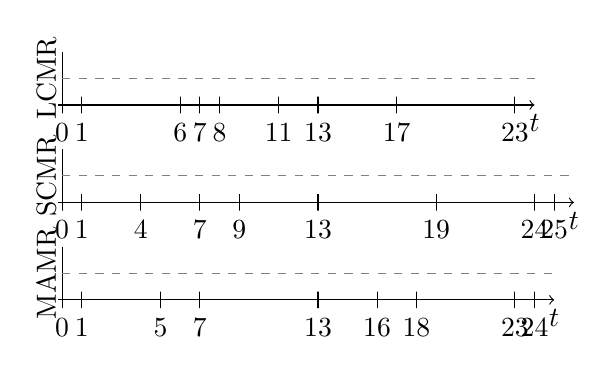
\begin{tikzpicture}[yscale=0.45,xscale=0.25]
			\begin{scope}
			\schedule{24}{LCMR}{1,6,7,8,11,13,17,23}
			\taskB{0}
			\taskD[1]{1}
			\taskA{8}
			\taskC{13}
			\end{scope}
			\begin{scope}[yshift=-2.75cm]
			\schedule{26}{SCMR}{1,4,7,9,13,19,24,25}
			\taskB{0}
			\taskA[3]{1}
			\taskC{9}
			\taskD{19}
			\end{scope}
			\begin{scope}[yshift=-5.5cm]
			\schedule{25}{MAMR}{1,5,7,13,16,18,23,24}
			\taskB{0}
			\taskC[2]{1}
			\taskA{13}
			\taskD{18}
			\end{scope}
	\end{tikzpicture}
		\end{block}
		
	\end{column}
\end{columns}
\end{frame}

\subsection{Static Order with Dynamic Corrections Based Strategies}
\begin{frame}{Static Order with Dynamic Corrections Based Strategies}
\begin{itemize}
	\vfill
	\item \textit{optimal order infinite memory largest communication task respects memory restriction} ($OOLCMR$)
	\vfill
	\item \textit{optimal order infinite memory smallest communication task respects memory restriction} ($OOSCMR$)
	\vfill
	\item \textit{optimal order infinite memory maximum accelerated task respects memory restriction} ($OOMAMR$)
	\vfill
\end{itemize}
\end{frame}

\begin{frame}{Static Order with Dynamic Corrections Based Strategies}
\begin{columns}
	\footnotesize
	\begin{column}[c]{0.4\linewidth}
		\begin{tabular}{|c|c|c|c|}
			\hline
	Task & Memory & Comm & Comp\\
& Req & Time & Time\\ \hline 
			%%			\multirow{2}{*}{Task} & Memory Req & \multirow{2}{*}{Comm Time} & \multirow{2}{*}{Comp Time}\\  
			%%			&=Comm Volume && \\ \hline
			A & 4 & 4 &  1\\ \hline
			B & 2 & 2 & 6\\ \hline
			C & 8 & 8 & 8\\ \hline
			D & 5 & 5 & 4\\ \hline
			E & 3 & 3 & 2\\ \hline
		\end{tabular}
	\end{column}
	\begin{column}[c]{0.6\linewidth}
		\begin{block}{Memory Capacity=9}
%%\newcommand{\taskA}[2][0]{\task[#1]{$A$}{#2}{4}{1}{cyan}}
%%\newcommand{\taskB}[2][0]{\task[#1]{$B$}{#2}{2}{6}{cyan!50!black}}
%%\newcommand{\taskC}[2][0]{\task[#1]{$C$}{#2}{8}{8}{blue!40!white}}
%%\newcommand{\taskD}[2][0]{\task[#1]{$D$}{#2}{5}{4}{blue!70!white}}
%%\newcommand{\taskE}[2][0]{\task[#1]{$E$}{#2}{3}{2}{blue}}
\newcommand{\taskA}[2][0]{\task[####1]{$A$}{####2}{4}{1}{cyan}}
\newcommand{\taskB}[2][0]{\task[####1]{$B$}{####2}{2}{6}{cyan!50!black}}
\newcommand{\taskC}[2][0]{\task[####1]{$C$}{####2}{8}{8}{blue!40!white}}
\newcommand{\taskD}[2][0]{\task[####1]{$D$}{####2}{5}{4}{blue!70!white}}
\newcommand{\taskE}[2][0]{\task[####1]{$E$}{####2}{3}{2}{blue}}
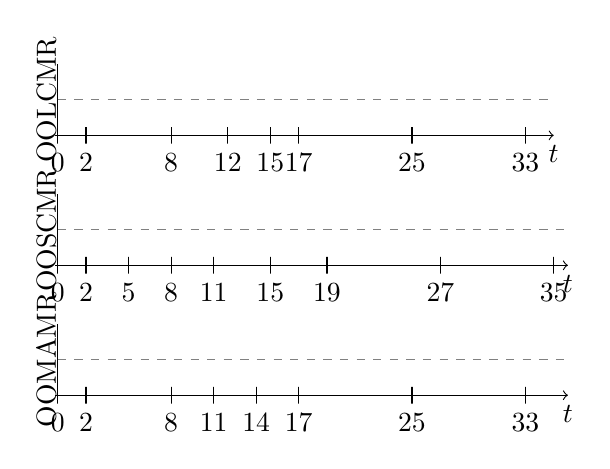
\begin{tikzpicture}[yscale=0.6,xscale=0.18]
\begin{scope}
\schedule{35}{OOLCMR}{2,8,12,15,17,25,33}
\taskB{0}
\taskD[1]{2}
\taskA{8}
\taskE{12}
\taskC{17}
\end{scope}
\begin{scope}[yshift=-2.75cm]
\schedule{36}{OOSCMR}{2,5,8,11,15,19,27,35}
\taskB{0}
\taskE[3]{2}
\taskA[1]{5}
\taskD{10}
\taskC{19}
\end{scope}
\begin{scope}[yshift=-5.5cm]
\schedule{36}{OOMAMR}{2,8,11,14,17,25,33}
\taskB{0}
\taskD[1]{2}
\taskE[1]{8}
\taskA{12}
\taskC{17}
\end{scope}
\end{tikzpicture}
		\end{block}
	\end{column}	
\end{columns}
\end{frame}


\begin{frame}{Favorable Situations for Heuristics}
\scriptsize
%%\vspace*{-0.5cm}
\begin{center}
\begin{tabular}{|c|p{9 cm}|}
	\hline
	\textbf{Heuristic} & \textbf{\hspace{2cm}Favorable Situation} \\ \hline
	$OOSIM$ & Memory capacity is not a restriction (\textcolor{green}{Optimal}) \\ \hline
	$IOCMS$ & Memory capacity is not a restriction and tasks are compute intensive (\textcolor{green}{Optimal}) \\ \hline
	$DOCPS$ & Memory capacity is not a restriction and tasks are communication intensive (\textcolor{green}{Optimal}) \\ \hline
	$IOCCS$ & Moderate memory capacity and most tasks are highly compute intensive \\ \hline
	$DOCCS$ & Moderate memory capacity and most tasks are highly communication intensive \\ \hline
	$LCMR$ & Limited memory capacity and significant percentage of tasks with large communication times are compute intensive\\ \hline
	$SCMR$ & Limited memory capacity and significant percentage of tasks with small communication times are compute intensive\\ \hline
	$MAMR$ & Limited memory capacity and significant percentage of all types of tasks\\ \hline
	$OOLCMR$ & Moderate memory capacity and significant percentage of slightly communication intensive tasks have large communication times\\ \hline
	$OOSCMR$ & Moderate memory capacity and significant percentage of slightly communication intensive tasks have small communication times\\ \hline
	$OOMAMR$ & Moderate memory capacity and significant percentage of all types of tasks \\ \hline
\end{tabular}
\end{center}
\end{frame}


\begin{frame}{Additional Heuristics from Previous Work}
\begin{block}{\textit{Gilmore-Gomory} ($GG$)}
	\begin{itemize}
		\item A classical algorithm for 2-machine no-wait flowshop problem
		\item Problem is represented by a graph
		\item An optimal sequence of vertices is obtained 
		\item Does not take memmory constraints into account
	\end{itemize}
\end{block}


\begin{block}{\textit{Bin Packing} ($BP$)}
	\begin{itemize}
		\item First-Fit algorithm for the bin packing problem
		\item Tasks added to the first bin in which they fit
		\item If no bin is found then a new bin is created
		\item Sequence made of all tasks from consecutive bins
	\end{itemize}
\end{block}
\end{frame}



\section{Workloads \& Hardware Configurations}
\begin{frame}
\frametitle{Table of Contents}
\tableofcontents[currentsection]
\end{frame}
\begin{frame}{Workload Characteristics}
\begin{block}{Molecular Chemistry Kernels}
\begin{itemize}
	\item 	Hartree--Fock (HF)  with SiOSi molecules and Coupled Cluster Singles Doubles (CCSD) with Uracil molecules
	\item Tensor operations: transpose and contraction
\end{itemize}
\end{block}
%%\begin{columns}
%%	\begin{column}[c]{0.5\linewidth}
%%		\includegraphics[scale=0.48]{./results/application_properties.pdf}
%%	\end{column}
%%\begin{column}[c]{0.5\linewidth}
%%\end{column}
%%\end{columns}

	\begin{block}{}
	\begin{center}
		\includegraphics[scale=0.5]{./diagrams/results/application_properties.pdf}
%%		\includegraphics[scale=0.48]{./diagrams/results/test1.pdf}
	\end{center}
	\end{block}

\end{frame}

\begin{frame}{Configuration Parameters to Obtain Traces}
\begin{itemize}
	\item 10 nodes of Cascade machine
	\item Each node contains 16 Intel Xeon E5-2670 cores
	\item Double precision version of  HF and CCSD of NWChem
	\item NWChem takes advantages of Global Arrays (GA) 
%%	a Partitioned Global Address Space Programming Model -- Global Arrays (GA)
	\item 150 processes for each application,  300-800 tasks for each process

\end{itemize}

\begin{block}{Simulation Parameters}
\begin{itemize}
	\item $m_c$: minimum memory capacity requirement to execute all tasks of an application
	\item Evaluation criteria for a heuristic $H$, $r(H)=\frac{\text{makespan of $H$}}{OMIM}$ (lower values are better)
	\item All data transfers between the local memory of each process and the GA memory take the same route
%%	\item Only one route for the same source-destination pair
\end{itemize}
\end{block}
\end{frame}


\begin{frame}{HF Performance with $m_c=176KB$.}
%%			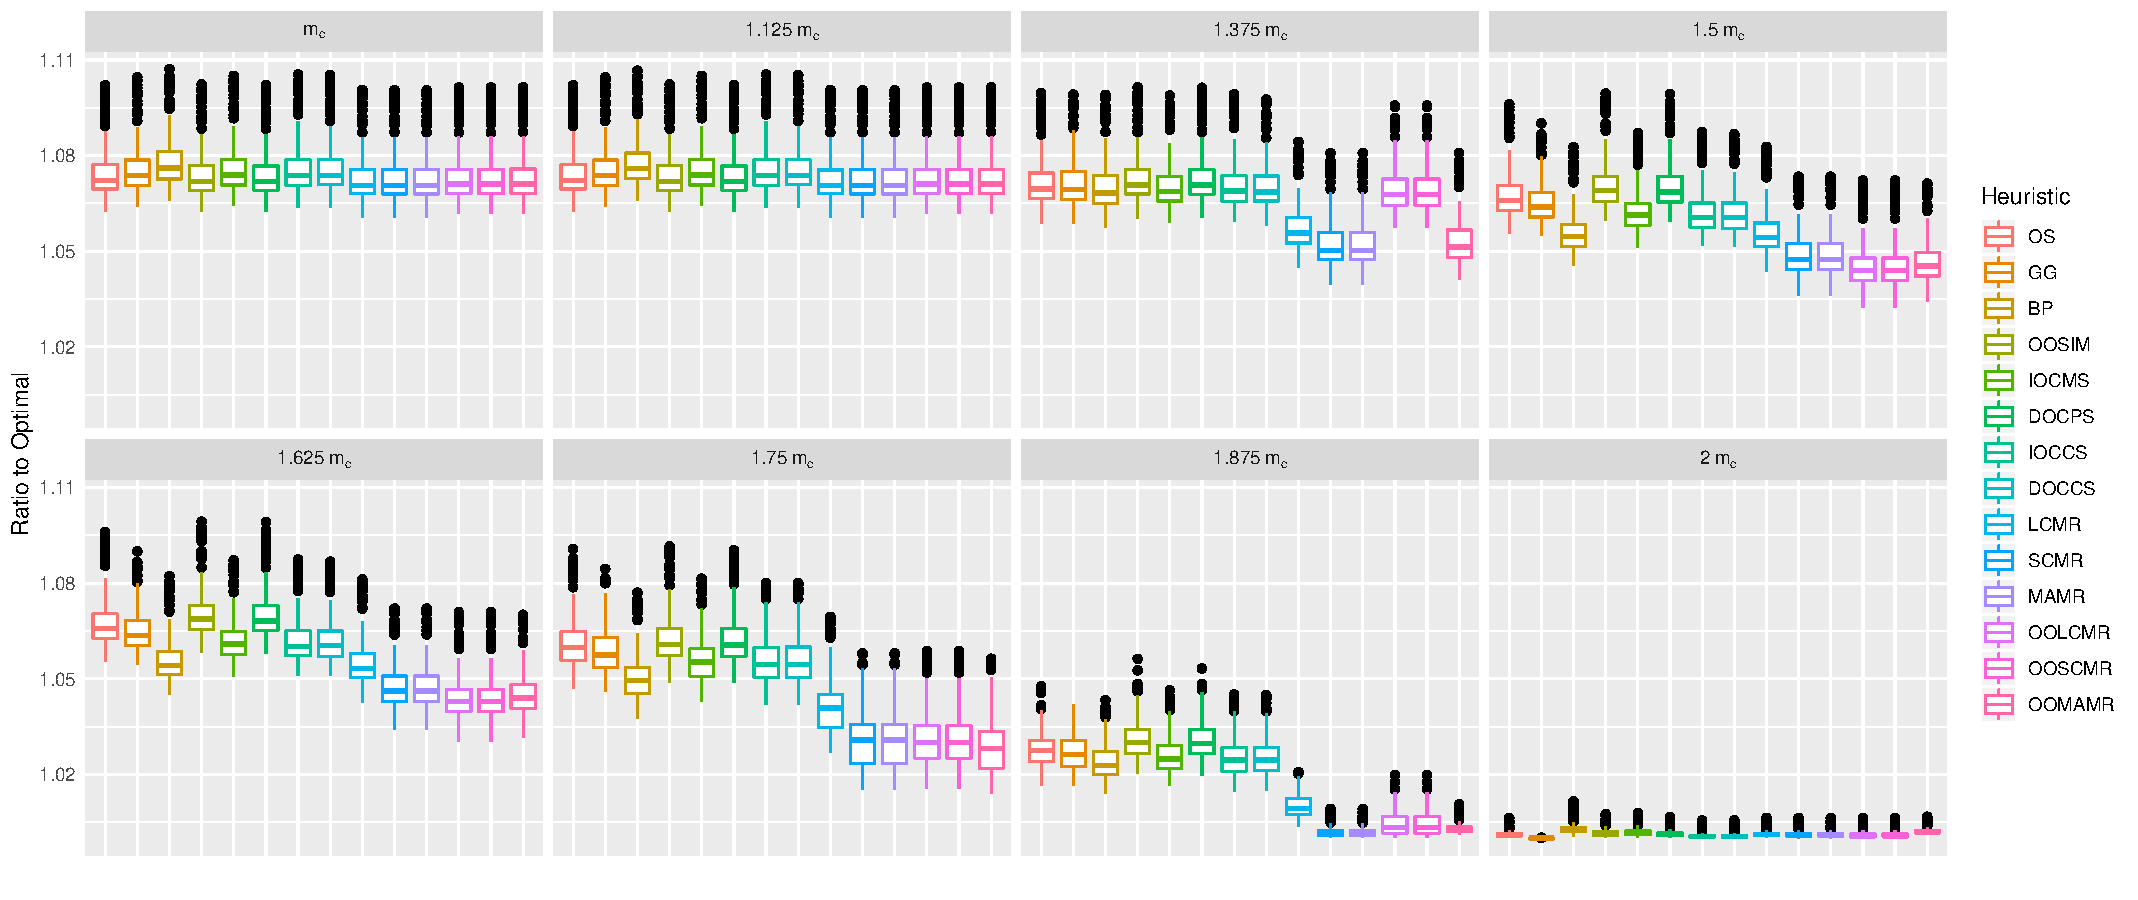
\includegraphics[scale=0.5]{./diagrams/results/ratio_to_optimal_selected_hf.pdf}
\begin{center}
%%			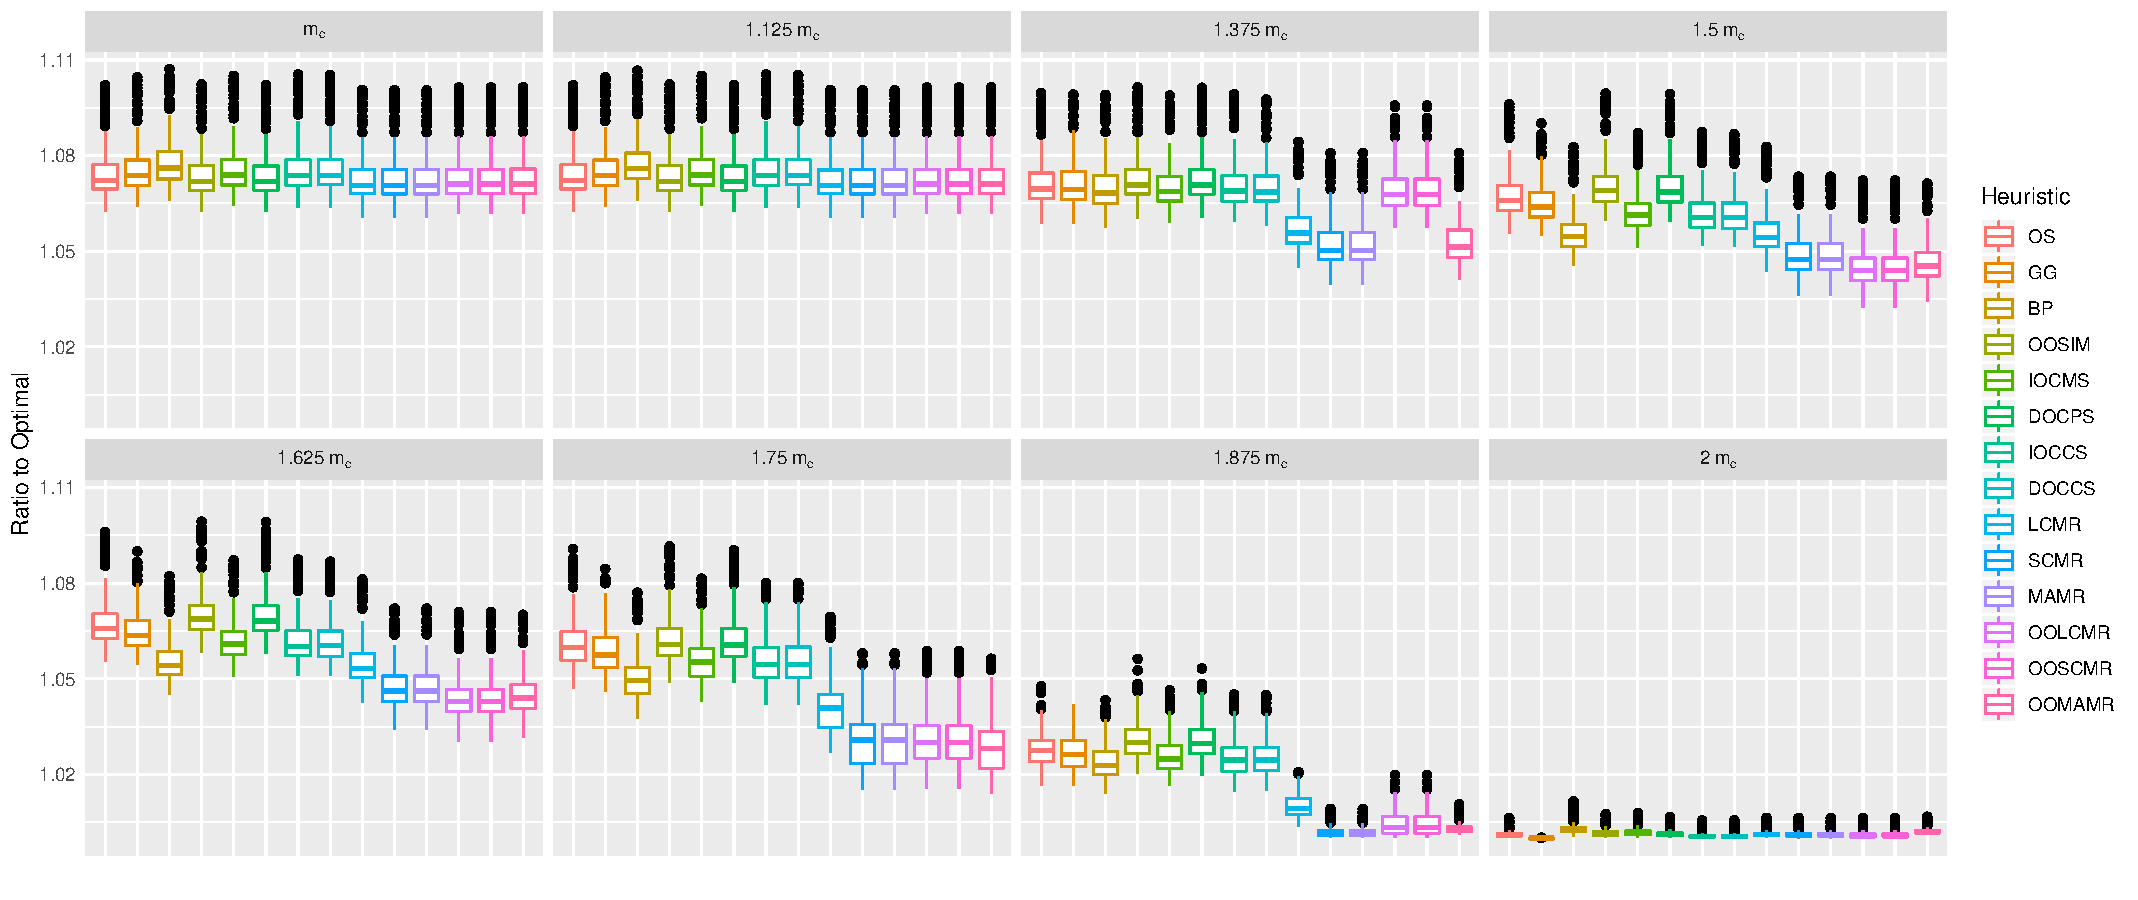
\includegraphics[scale=0.335]{./diagrams/results/ratio_to_optimal_selected_hf.pdf}
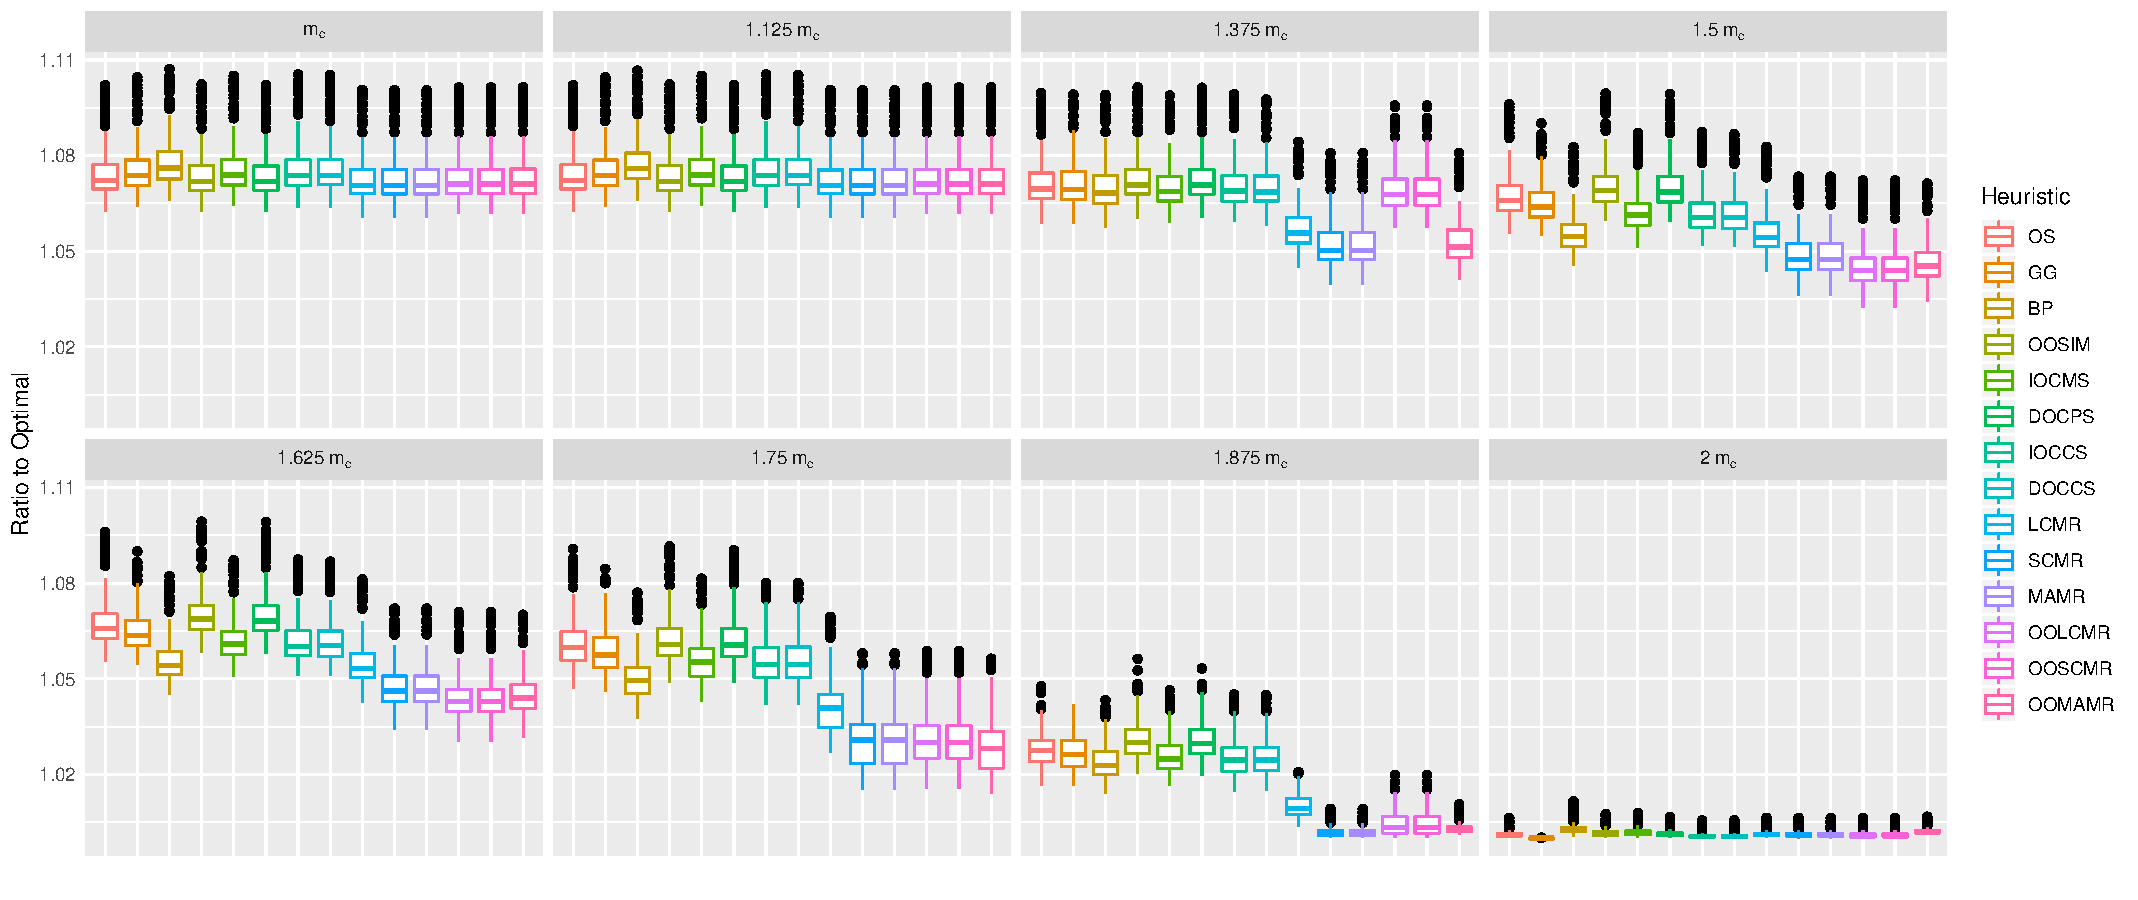
\includegraphics[width=1.05\linewidth]{./diagrams/results/ratio_to_optimal_selected_hf.pdf}
%%	\includegraphics[scale=0.335]{./diagrams/results/test1.pdf}
\end{center}
$\bullet$ Dynamic strategies are best suited for limited memory capacities\\
$\bullet$ Static order with dynamic correction variants outperform others for moderate memory capacities
\end{frame}

\begin{frame}{CCSD performance with $m_c=1.8GB$}
\begin{center}
	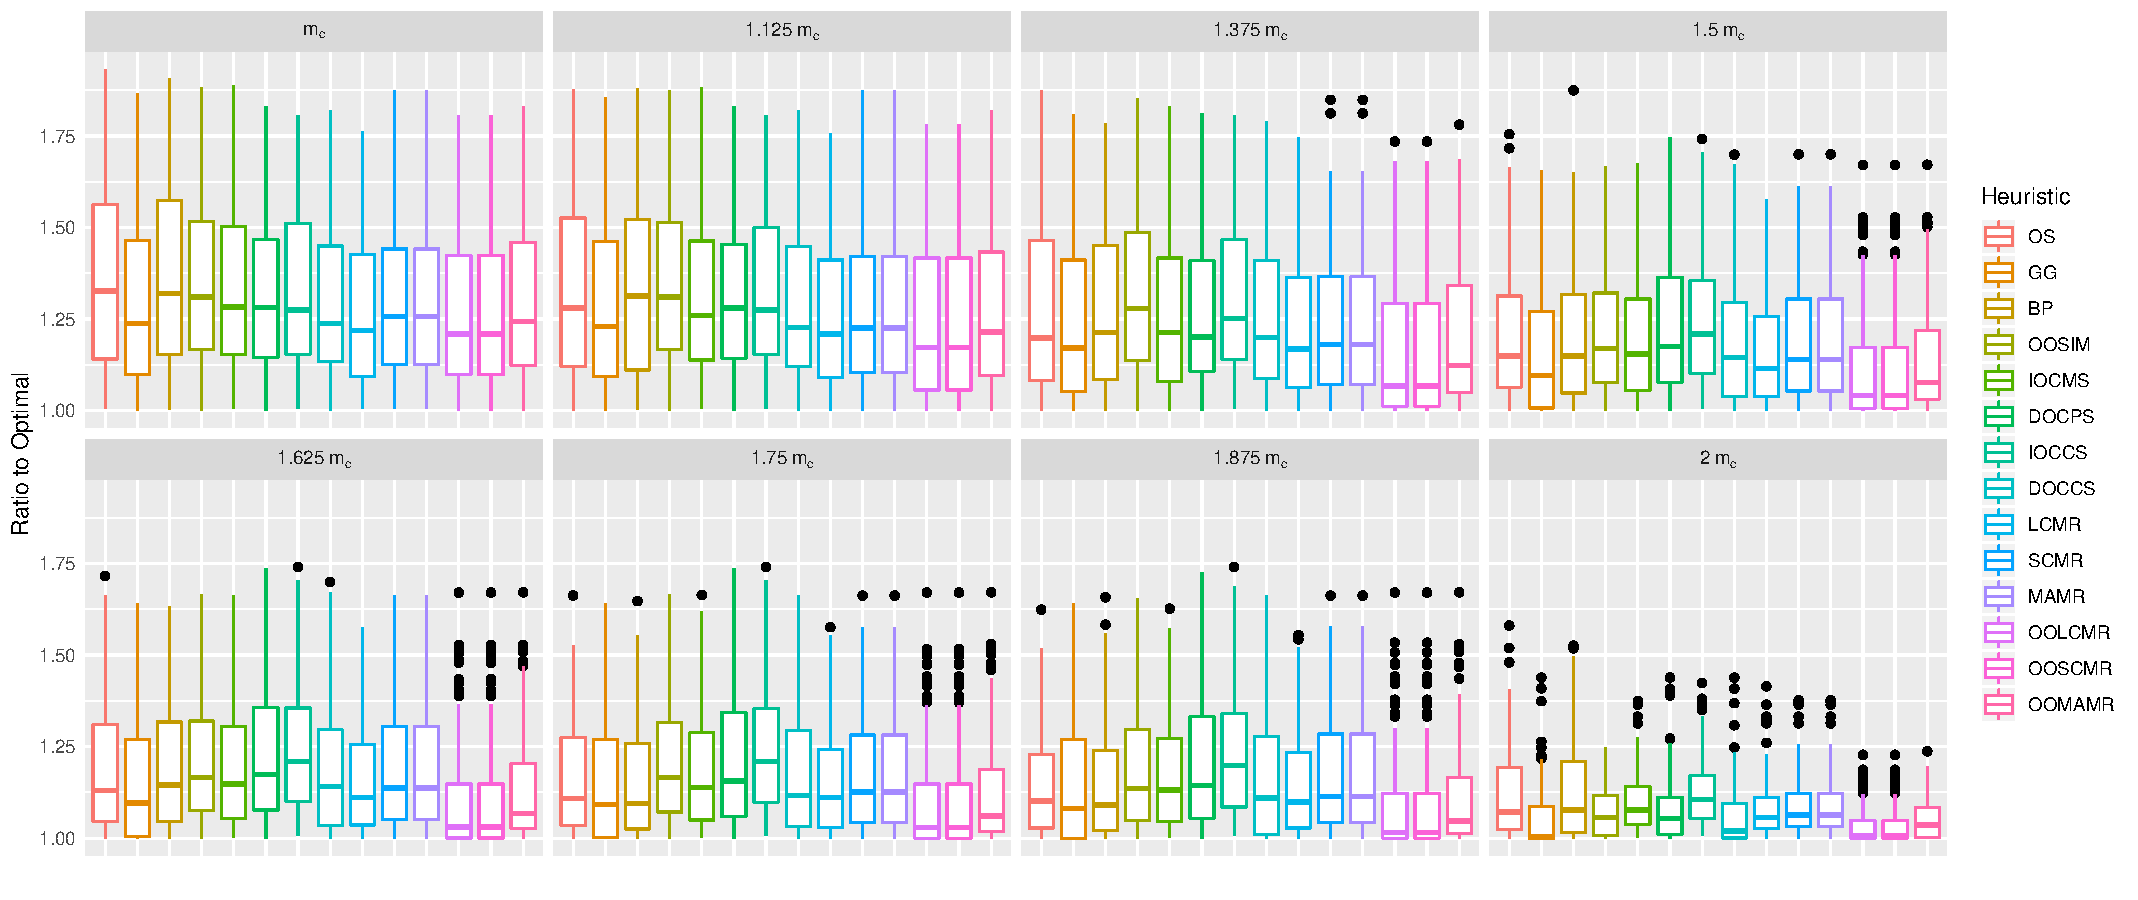
\includegraphics[width=1.05\linewidth]{./diagrams/results/ratio_to_optimal_selected_ccsd.pdf}
\end{center}
$\bullet$ Highly heterogeneous tasks\\
$\bullet$ Static order with dynamic correction variants outperform others in most cases
\end{frame}

\begin{frame}{Best variants of all categories}
%%\begin{columns}
%%	\begin{column}{0.55\linewidth}
\begin{block}{\only<1>{HF} \only<2>{CCSD} Performance}
	\begin{center}
\only<1>{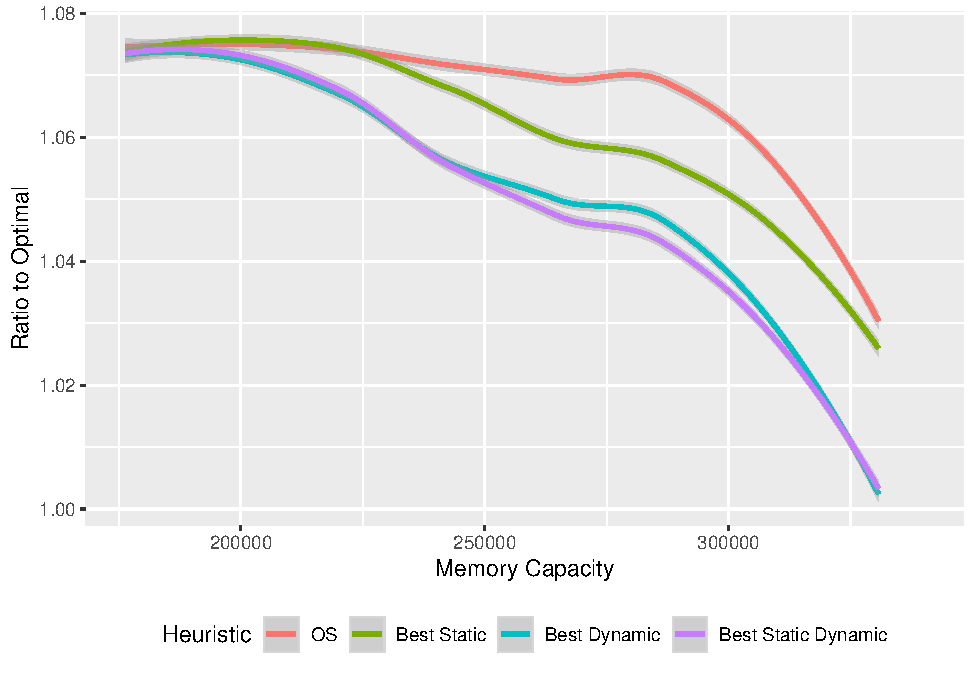
\includegraphics[width=0.85\linewidth]{./diagrams/results/ratio_to_optimal_hf-best.pdf}}
\only<2>{\includegraphics[width=0.85\linewidth]{./diagrams/results/ratio_to_optimal_ccsd-best.pdf}}
	\end{center}
\end{block}
\end{frame}

\begin{frame}{Implementation challenges}
\begin{itemize}
	\vfill
	\item Impact of Congestion on communication/computation times
	\vfill
	\item Output data of a task
	\vfill
	\item Routes between two memory nodes
	\vfill
	\item Communications from multiple memory nodes can happen at the same time
	\vfill
\end{itemize}
\end{frame}


 \section{Conclusion and Ongoing Work}
 \begin{frame}
\frametitle{Table of Contents}
\tableofcontents[currentsection]
\end{frame}
 \begin{frame}{Conclusion and Ongoing Work}
Conclusion:
 \begin{itemize}
  \item Problem of determining the optimal order of data transfers is NP-complete
  \item Our heuristics achieve significant overlap for HF and CCSD applications
 \end{itemize}
\vfill
Ongoing work: 
%% \end{frame}
%% \begin{frame}{Future work}
 \begin{itemize}
  \item Evaluation of our heuristics in the context of accelerators
  \item Implementation of the proposed heuristics
 \item Automatic selection of the best heuristic
 \item Model bandwidth sharing to support multiple simultaneous communications
 \end{itemize}
 \end{frame}


%% \begin{frame}
%%  \begin{center}
%%   {\huge Thank \newline You!}
%%    
%%  \end{center}
%% \end{frame}

\end{document}




